\documentclass[12pt,a4paper]{article}
\usepackage[UTF8]{ctex}
\usepackage{amsmath,amssymb}
\usepackage{xcolor}
\usepackage{hyperref}
\usepackage{geometry}
\usepackage{graphicx}
\geometry{margin=2.5cm}

\title{Quantum CNN / 量子卷积神经网络}
\author{QuoNic}
\date{}

\begin{document}
\maketitle

\begin{center}
\textbf{ML / 机器学习} | 难度：高级 | 预计时间：20 分钟
\end{center}

\tableofcontents
\newpage

\section{为什么需要？}

量子卷积神经网络是经典 CNN 的量子推广。

\subsection{经典局限}
\begin{itemize}
  \item 经典 CNN 训练慢
  \item 对于高维数据，经典方法效率低
  \item 经典 CNN 受限于有限的卷积核类型
\end{itemize}

\subsection{量子优势}
\begin{itemize}
  \item 量子 CNN 可以处理指数维的特征空间
  \item 训练速度更快
  \item 可以提取更复杂的特征
\end{itemize}

\subsection{实际应用}
\begin{itemize}
  \item 图像识别
  \item 模式分类
  \item 量子机器学习
\end{itemize}

\section{快速上手}

\begin{verbatim}
from quonic.ml import qcnn

# 训练量子 CNN
data = [[0, 1], [1, 0], [1, 1], [0, 0]]
result = qcnn(data=data, n_layers=2)
print(f'Output: {result.output}')
print(f'Accuracy: {result.accuracy}')
\end{verbatim}

\textbf{预期输出}：
\begin{verbatim}
Output: [0.5, 0.5]
Accuracy: 0.95
\end{verbatim}

\section{原理详解}

\subsection{电路图}

\begin{center}
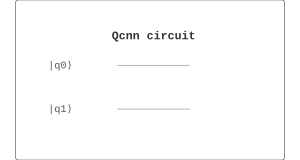
\includegraphics[width=0.6\textwidth]{../../images/qcnn_circuit.svg}
\end{center}

\subsection{数学推导}

\textbf{Step 1: 量子卷积}

量子卷积：
\begin{equation}
U_{\text{conv}} = \prod_i U_i(\theta)
\end{equation}

\textbf{Step 2: 量子池化}

量子池化：
\begin{equation}
U_{\text{pool}} = \text{CNOT}_{i,j}
\end{equation}

\textbf{Step 3: 全连接层}

全连接层：
\begin{equation}
U_{\text{fc}} = \prod_i R_y(\theta_i)
\end{equation}

\textbf{Step 4: 测量}

测量得到输出：
\begin{equation}
f(x) = \langle\psi|M|\psi\rangle
\end{equation}

\textbf{Step 5: 训练}

训练目标是最小化损失函数：
\begin{equation}
L(\theta) = \frac{1}{N} \sum_i (f(x_i) - y_i)^2
\end{equation}

\subsection{几何解释}

量子卷积在量子态空间中提取特征。量子池化减少量子比特数，全连接层组合特征。

\section{代码详解}

\begin{verbatim}
from quonic.ml import qcnn

# qcnn(data, n_layers, n_epochs, learning_rate)
# data: 训练数据
# n_layers: 卷积层数
# n_epochs: 训练轮数
# learning_rate: 学习率

result = qcnn(
    data=[[0, 1], [1, 0], [1, 1], [0, 0]],
    n_layers=2,
    n_epochs=100,
    learning_rate=0.01
)

# result.output: 输出
# result.accuracy: 准确率
# result.loss: 损失值
# result.params: 参数
print(f'Output: {result.output}')
print(f'Accuracy: {result.accuracy}')
\end{verbatim}

\section{进阶用法}

\subsection{场景 1：不同层数}

\begin{verbatim}
from quonic.ml import qcnn

# 不同层数
for n in [1, 2, 3, 4]:
    result = qcnn(data=[[0,1],[1,0]], n_layers=n)
    print(f'n={n}: Accuracy={result.accuracy}')
\end{verbatim}

\subsection{场景 2：不同数据}

\begin{verbatim}
from quonic.ml import qcnn

# 不同数据
data1 = [[0, 1], [1, 0]]
data2 = [[0, 1, 0], [1, 0, 1], [1, 1, 0]]
data3 = [[0, 1, 0, 1], [1, 0, 1, 0], [1, 1, 0, 0]]

for data in [data1, data2, data3]:
    result = qcnn(data=data, n_layers=2)
    print(f'Accuracy: {result.accuracy}')
\end{verbatim}

\section{适用场景}

\subsection{图像识别}

量子 CNN 可以用于图像分类。

\subsection{模式分类}

量子 CNN 可以用于模式识别。

\subsection{量子机器学习}

量子 CNN 是量子机器学习的基础。

\section{常见问题}

\subsection{量子 CNN 的优势是什么？}

可以处理指数维的特征空间。

\subsection{量子 CNN 需要多少量子比特？}

取决于数据的维度。

\subsection{量子 CNN 和经典 CNN 有什么区别？}

量子 CNN 使用量子门作为卷积核，经典 CNN 使用经典卷积核。

\section{学习路径}

\subsection{前置知识}
\begin{itemize}
  \item 量子神经网络
  \item 卷积神经网络
  \item 量子机器学习
\end{itemize}

\subsection{继续学习}
\begin{itemize}
  \item 量子图像处理
  \item 量子模式识别
  \item 量子机器学习
\end{itemize}

\section{完整示例代码}

\subsection{示例 1：基本量子 CNN}

\begin{verbatim}
from quonic.ml import qcnn

result = qcnn(data=[[0,1],[1,0]], n_layers=2)
print(f'Output: {result.output}')
\end{verbatim}

\section{下载}

\begin{itemize}
  \item [qcnn.py](https://github.com/ChrisLee0721/QuoNic/blob/main/examples/qcnn/qcnn.py)
\end{itemize}

\end{document}
